% Options for packages loaded elsewhere
\PassOptionsToPackage{unicode}{hyperref}
\PassOptionsToPackage{hyphens}{url}
%
\documentclass[
  man,floatsintext]{apa7}
\usepackage{amsmath,amssymb}
\usepackage{iftex}
\ifPDFTeX
  \usepackage[T1]{fontenc}
  \usepackage[utf8]{inputenc}
  \usepackage{textcomp} % provide euro and other symbols
\else % if luatex or xetex
  \usepackage{unicode-math} % this also loads fontspec
  \defaultfontfeatures{Scale=MatchLowercase}
  \defaultfontfeatures[\rmfamily]{Ligatures=TeX,Scale=1}
\fi
\usepackage{lmodern}
\ifPDFTeX\else
  % xetex/luatex font selection
\fi
% Use upquote if available, for straight quotes in verbatim environments
\IfFileExists{upquote.sty}{\usepackage{upquote}}{}
\IfFileExists{microtype.sty}{% use microtype if available
  \usepackage[]{microtype}
  \UseMicrotypeSet[protrusion]{basicmath} % disable protrusion for tt fonts
}{}
\makeatletter
\@ifundefined{KOMAClassName}{% if non-KOMA class
  \IfFileExists{parskip.sty}{%
    \usepackage{parskip}
  }{% else
    \setlength{\parindent}{0pt}
    \setlength{\parskip}{6pt plus 2pt minus 1pt}}
}{% if KOMA class
  \KOMAoptions{parskip=half}}
\makeatother
\usepackage{xcolor}
\usepackage{graphicx}
\makeatletter
\def\maxwidth{\ifdim\Gin@nat@width>\linewidth\linewidth\else\Gin@nat@width\fi}
\def\maxheight{\ifdim\Gin@nat@height>\textheight\textheight\else\Gin@nat@height\fi}
\makeatother
% Scale images if necessary, so that they will not overflow the page
% margins by default, and it is still possible to overwrite the defaults
% using explicit options in \includegraphics[width, height, ...]{}
\setkeys{Gin}{width=\maxwidth,height=\maxheight,keepaspectratio}
% Set default figure placement to htbp
\makeatletter
\def\fps@figure{htbp}
\makeatother
\setlength{\emergencystretch}{3em} % prevent overfull lines
\providecommand{\tightlist}{%
  \setlength{\itemsep}{0pt}\setlength{\parskip}{0pt}}
\setcounter{secnumdepth}{-\maxdimen} % remove section numbering
% Make \paragraph and \subparagraph free-standing
\ifx\paragraph\undefined\else
  \let\oldparagraph\paragraph
  \renewcommand{\paragraph}[1]{\oldparagraph{#1}\mbox{}}
\fi
\ifx\subparagraph\undefined\else
  \let\oldsubparagraph\subparagraph
  \renewcommand{\subparagraph}[1]{\oldsubparagraph{#1}\mbox{}}
\fi
\newlength{\cslhangindent}
\setlength{\cslhangindent}{1.5em}
\newlength{\csllabelwidth}
\setlength{\csllabelwidth}{3em}
\newlength{\cslentryspacingunit} % times entry-spacing
\setlength{\cslentryspacingunit}{\parskip}
\newenvironment{CSLReferences}[2] % #1 hanging-ident, #2 entry spacing
 {% don't indent paragraphs
  \setlength{\parindent}{0pt}
  % turn on hanging indent if param 1 is 1
  \ifodd #1
  \let\oldpar\par
  \def\par{\hangindent=\cslhangindent\oldpar}
  \fi
  % set entry spacing
  \setlength{\parskip}{#2\cslentryspacingunit}
 }%
 {}
\usepackage{calc}
\newcommand{\CSLBlock}[1]{#1\hfill\break}
\newcommand{\CSLLeftMargin}[1]{\parbox[t]{\csllabelwidth}{#1}}
\newcommand{\CSLRightInline}[1]{\parbox[t]{\linewidth - \csllabelwidth}{#1}\break}
\newcommand{\CSLIndent}[1]{\hspace{\cslhangindent}#1}
\ifLuaTeX
\usepackage[bidi=basic]{babel}
\else
\usepackage[bidi=default]{babel}
\fi
\babelprovide[main,import]{english}
% get rid of language-specific shorthands (see #6817):
\let\LanguageShortHands\languageshorthands
\def\languageshorthands#1{}
% Manuscript styling
\usepackage{upgreek}
\captionsetup{font=singlespacing,justification=justified}

% Table formatting
\usepackage{longtable}
\usepackage{lscape}
% \usepackage[counterclockwise]{rotating}   % Landscape page setup for large tables
\usepackage{multirow}		% Table styling
\usepackage{tabularx}		% Control Column width
\usepackage[flushleft]{threeparttable}	% Allows for three part tables with a specified notes section
\usepackage{threeparttablex}            % Lets threeparttable work with longtable

% Create new environments so endfloat can handle them
% \newenvironment{ltable}
%   {\begin{landscape}\centering\begin{threeparttable}}
%   {\end{threeparttable}\end{landscape}}
\newenvironment{lltable}{\begin{landscape}\centering\begin{ThreePartTable}}{\end{ThreePartTable}\end{landscape}}

% Enables adjusting longtable caption width to table width
% Solution found at http://golatex.de/longtable-mit-caption-so-breit-wie-die-tabelle-t15767.html
\makeatletter
\newcommand\LastLTentrywidth{1em}
\newlength\longtablewidth
\setlength{\longtablewidth}{1in}
\newcommand{\getlongtablewidth}{\begingroup \ifcsname LT@\roman{LT@tables}\endcsname \global\longtablewidth=0pt \renewcommand{\LT@entry}[2]{\global\advance\longtablewidth by ##2\relax\gdef\LastLTentrywidth{##2}}\@nameuse{LT@\roman{LT@tables}} \fi \endgroup}

% \setlength{\parindent}{0.5in}
% \setlength{\parskip}{0pt plus 0pt minus 0pt}

% Overwrite redefinition of paragraph and subparagraph by the default LaTeX template
% See https://github.com/crsh/papaja/issues/292
\makeatletter
\renewcommand{\paragraph}{\@startsection{paragraph}{4}{\parindent}%
  {0\baselineskip \@plus 0.2ex \@minus 0.2ex}%
  {-1em}%
  {\normalfont\normalsize\bfseries\itshape\typesectitle}}

\renewcommand{\subparagraph}[1]{\@startsection{subparagraph}{5}{1em}%
  {0\baselineskip \@plus 0.2ex \@minus 0.2ex}%
  {-\z@\relax}%
  {\normalfont\normalsize\itshape\hspace{\parindent}{#1}\textit{\addperi}}{\relax}}
\makeatother

% \usepackage{etoolbox}
\makeatletter
\patchcmd{\HyOrg@maketitle}
  {\section{\normalfont\normalsize\abstractname}}
  {\section*{\normalfont\normalsize\abstractname}}
  {}{\typeout{Failed to patch abstract.}}
\patchcmd{\HyOrg@maketitle}
  {\section{\protect\normalfont{\@title}}}
  {\section*{\protect\normalfont{\@title}}}
  {}{\typeout{Failed to patch title.}}
\makeatother

\usepackage{xpatch}
\makeatletter
\xapptocmd\appendix
  {\xapptocmd\section
    {\addcontentsline{toc}{section}{\appendixname\ifoneappendix\else~\theappendix\fi\\: #1}}
    {}{\InnerPatchFailed}%
  }
{}{\PatchFailed}
\keywords{keyword, more keyword, crazy keyword\newline\indent Word count: X}
\usepackage{csquotes}
\makeatletter
\renewcommand{\paragraph}{\@startsection{paragraph}{4}{\parindent}%
  {0\baselineskip \@plus 0.2ex \@minus 0.2ex}%
  {-1em}%
  {\normalfont\normalsize\bfseries\typesectitle}}

\renewcommand{\subparagraph}[1]{\@startsection{subparagraph}{5}{1em}%
  {0\baselineskip \@plus 0.2ex \@minus 0.2ex}%
  {-\z@\relax}%
  {\normalfont\normalsize\bfseries\itshape\hspace{\parindent}{#1}\textit{\addperi}}{\relax}}
\makeatother

\raggedbottom

\usepackage{hhline}

\setlength{\parskip}{0pt}

\ifLuaTeX
  \usepackage{selnolig}  % disable illegal ligatures
\fi
\IfFileExists{bookmark.sty}{\usepackage{bookmark}}{\usepackage{hyperref}}
\IfFileExists{xurl.sty}{\usepackage{xurl}}{} % add URL line breaks if available
\urlstyle{same}
\hypersetup{
  pdftitle={An algorithm for detecting ERP components using the grand average waveform as a template},
  pdfauthor={Sven Lesche1},
  pdflang={en-EN},
  pdfkeywords={keyword, more keyword, crazy keyword},
  hidelinks,
  pdfcreator={LaTeX via pandoc}}

\title{An algorithm for detecting ERP components using the grand average waveform as a template}
\author{Sven Lesche\textsuperscript{1}}
\date{}


\shorttitle{Template Matching}

\authornote{

Author Notes go here.

The authors made the following contributions. Sven Lesche: Conceptualization, Writing - Original Draft Preparation, Writing - Review \& Editing.

Correspondence concerning this article should be addressed to Sven Lesche, Im Neuenheimer Feld 695, 69120 Heidelberg. E-mail: \href{mailto:sven.lesche@psychologie.uni-heidelberg.de}{\nolinkurl{sven.lesche@psychologie.uni-heidelberg.de}}

}

\affiliation{\vspace{0.5cm}\textsuperscript{1} Ruprecht-Karls-University Heidelberg}

\abstract{%
One or two sentences providing a \textbf{basic introduction} to the field, comprehensible to a scientist in any discipline.

Two to three sentences of \textbf{more detailed background}, comprehensible to scientists in related disciplines.

One sentence clearly stating the \textbf{general problem} being addressed by this particular study.

One sentence summarizing the main result (with the words ``\textbf{here we show}'' or their equivalent).

Two or three sentences explaining what the \textbf{main result} reveals in direct comparison to what was thought to be the case previously, or how the main result adds to previous knowledge.

One or two sentences to put the results into a more \textbf{general context}.

Two or three sentences to provide a \textbf{broader perspective}, readily comprehensible to a scientist in any discipline.
}



\begin{document}
\maketitle

\#exp28 \#EEG \#methods \#template

talk about the importance of erp latency extraction

talk about previous approaches and their problems: see {[}{[}outline template matching{]}{]}, and {[}{[}Issues with current latency measures{]}{]}

\hypertarget{relevance-of-erps}{%
\section{Relevance of ERPs}\label{relevance-of-erps}}

Event-related potentials (ERPs) are a key tool used in a variety of fields of study. Clinical psychology {[}REF{]}, cognitive psychology {[}REF{]}, experimental psychology {[}REF{]} all make use of ERPs to investigate the neural processes. Both the amplitude as well as the latency of components are often used to gain insights into individual differences in cognitive processes {[}REF{]}. Accurate estimation of the latency of ERP components thus presents an important topic relevant to all applications of ERP research {[}REF{]}.

\textbf{something about N2 and P3 processes here} \textbf{also write something about its relevance for individual differences research}

\textbf{the first paragraph should already illustrate how imporant accurate latency extraction methods are}

A number of algorithms have been developed hoping to ease identification of components and their latencies. The earliest version of an algorithm to automatically extract ERP latencies is the \emph{peak latency} approach {[}REF{]}. It involves finding the point in time within a set measurement window that has the largest voltage deflection in the appropriate direction. This method was developed as it was easy to implement \textbf{something about historical ease of use} \textbf{Luck, 2014, p.~286 cites Donchin \& Heffley, 1978 as historical example}. Even though an algorithm detecting the \emph{peak latency} inside some measurement window is easy to implement and run, it can be corrupted by several factors.

\textbf{be aware that luck lists the following issues: peak != component; high-freq noise; time-window/point differences in subjects; biased by noise-level; is non-linear measure; influence of latency jitter; difficult to compare with RT}

\begin{enumerate}
\def\labelenumi{\arabic{enumi}.}
\tightlist
\item
  Choice of measurement window
  As the peak latency method is blind to the general structure within the ERP signal, it simply chooses the point in time with the largest voltage deflection within the measurement window. The ``true'' maximum signal may lay just outside of the measurement window, resulting in the algorithm picking an outside edge of the window to reflect the \emph{peak latency}, even though the signal increases in amplitude just following that timepoint. This may be true even if there is a clear component-like structure fully contained in the measurement window. Later components may already influence the amplitude on the outer ranges of the measurement window, resulting in their latency being picked instead of the true component of interest. Simple \emph{peak latency} algorithms can thus fail to pick the \emph{local maximum} of a component of interest fully contained inside the measurement window in favor of a datapoint possibly influenced by later or earlier components. This problem is often referred to as the \emph{superimposition problem} {[}REF, just luck, 2014?{]}.
\end{enumerate}

To combat the influence of other components, {[}REF{]} have modified the simple \emph{peak latency} algorithm to only consider maxima inside the measurement window which are also larger than the surrounding datapoints. A spike just on the edge of the measurement window induced by a later component will not meet these criteria, as the last datapoint inside the measurement window will be smaller than the following datapoint. This method is more accurate in finding the \emph{local} peak latency {[}REF{]} but still vulnerable to other issues with peak latency approaches.

\begin{enumerate}
\def\labelenumi{\arabic{enumi}.}
\setcounter{enumi}{1}
\item
  Superimposition of other components
  The \emph{peak latency} approach is also especially vulnerable to influences of other components on the ERP signal - \textbf{bad sentence}. Even though the inclusion of neighboring datapoints does help the algorithms find local optima, peak latency approaches will fail to detect the peak of the component of interest if the measurement window contains portions of non-relevant components. Researchers thus have to carefully choose the measurement window in order to \textbf{not include other components}, \textbf{keep it homogenous across all subjects}, \textbf{fully include the component of interest}
\item
  high frequency noise
  The influence of high frequency noise presents another issue for peak latency algorithms. The maximum voltage deflection may not reflect the true point in time at which the component reaches its maximum. Rather it may be the result of high frequency noise inducing a spike in the signal, independent of any cognitive process. This is problematic especially in the identification of the latency of later ERP components, as the larger measurement window most commonly applied here will increase the likelihood of high frequency noise impacting the maximum voltage deflection {[}REF, luck? or liesemeier?{]}.
\item
  The peak latency is also just not that relevant
  Lastly, as {[}Luck, 2014{]} so aptly states: \emph{There is nothing special about the point at which the voltage reaches a local maximum}. The largest deflection does not inherently relate to any physiological or psychological process and may not even reflect the true maximum of the component of interest due to the \emph{superimposition problem}. {[}REF luck rule paper{]} visually demonstrates how peak latency may be a result of the overlap of multiple components and not related to any single component.
\end{enumerate}

\emph{Fractional Area Latency} approaches hope to remedy some of the problems associated with \emph{peak latency} algorithms. \emph{Fractional Area Latency} revolves around the area under the ERP signal in a given measurement window and finding the point in time that divides that area into a given fraction before and a after that point in time. The timepoint halving the area under the signal, for example, is referred to as the \emph{50\% area latency}. This approach is much less susceptible to the influence of high frequency noise, as short spikes in the signal do not influence the area under the signal much. It remains highly dependent on the measurement window {[}Luck, 2005{]}. Choosing a shorter window may result in only a part of the area of the component of interest being captured. A wider measurement window on the other hand might be influenced by surrounding components. \emph{Fractional Area} measures thus work best for investigating an isolated component {[}Luck, 2014{]}, limiting the applicability of algorithms based on this.

Another approach towards dealing with noisy subject-level ERPs is to try and remove that noise by averaging multiple subject-level ERPs. This technique is referred to as \emph{jackknifing}. It uses the grand average of \(N\) subject-level ERPs and generates \(N\) sub-grand averages by removing one of the subject-level ERPs from this grand average. This results in \(N\) ERPs with higher signal-to-noise ratios as they are the average of \(N-1\) subject-level ERPs. Both \emph{peak} and \emph{area} based measures can then be applied to the jackknifed data to extract latencies. As jackknifed signals share \(\frac{N-2}{N} * 100\) percent of the subject-level signals that are averaged, each jackknifed-subaverage is quite similar to all others. This artificially decreases the error variance, which needs to be corrected for when testing for significant differences between groups {[}(Ulrich \& Miller, 2001), aus Sadus (2023){]}. Because Latencies extracted from jackknifed ERPs are based on averaged waveforms, they can not be readily associated with any single subject, preventing this method from generating individual-level latency estimates needed for individual differences research. This problem was adressed by {[}Smulders 2010, aus Sadus (2023){]} who introduced a transformation able to generate individual-level latency estimates.

{[}Kiesel 2008{]} compared a number of extraction methods for a variety of ERP components and found {[}SUMMARY HERE{]}. Their analyses indicates \textbf{drawbacks of each method summarized}
{[}Sadus 2023{]} used a multiverse approach to investigate P3 stuff and utilizied \textbf{these} algorithms as well as manual extraction of ERP latencies \ldots{}

Look at comparison studies report what they thought is best. Sadus et al.~as last

the conclusion from this needs to be made clear: no algorithm provides a sufficiently reliable method of extracting component latencies. - Manual inspection seems to reign supreme, \textbf{talk about the practical problems associated with this}, \textbf{also talk about the methods problems, low objectivity}

When visually inspecting ERP signals, the goal is to identify a pattern within the signal that resembles the component of interest in shape, size and location. None of the previously described algorithms used in most ERP research aim to replicate this human behavior but rather focus on generating similar decisions, not similar decision processes. The goal of this work is to introduce a new method for extracting component latencies that more closely resembles the manual extraction process.

\textbf{pattern matching in short}
The general question each ERP-researcher asks themselves when investigating ERP signals is: ``Where in this ERP signal is the component of interest?'' Most researchers have some mental representation of what the component \emph{should} look like and where it \emph{should} generally appear that helps them identify a specific component in some noisy ERP.
Finding a given pattern inside a noisy signal is not a novel task in the field of signal processing. Algorithms aiming to detect the appearance of a pattern - a \emph{template} -inside audio-, video- or radio signals have been around since \textbf{HISTORY} {[}REF{]} and a large amount of research has gone into perfecting these \emph{template matching} algorithms {[}REF{]}.

No matter the implementation of the template matching algorithm, they all aim to answer the question ``Does this (shorter) template appear in my (larger) signal?''. To achieve this, a researcher needs to specify two things. First, the template that they want to search the signal for. And second, the \emph{deviance measure} by which the algorithm can figure out how well the template fits in a given spot of the signal.

Depending on the field, the first question is easily solved\ldots{} This was the problem for ERP research.
There has been some debate about the optimal answer to the second thing\ldots{} {[}REFs{]}

Our goal is to show that the concepts used in signal processing to find specific patterns can be adopted by ERP researchers to conduct \emph{template matching} in a similar manner.

There have been some attempts at using an idealized component structure, like the COMPONENT{[}depending on citation{]} and using template matching algorithms to identify the component in noisy subjet-level data. The variance of ERP signal structure within and especially between ERP studies has presented a challenge to this approach {[}REF{]}. The morphology of the P3, for example, varies depending on the task used and the participants studied {[}REF{]}. This compromises the ability to use a heavily idealized P3-like component as a template to search for in subject-level ERPs {[}Does it work with GA?{]}. \textbf{want to talk about the Hidden-semi-markov-chain approach?}

This problem can be addressed by using using an experiment-specific template of the component of interest that will reflect influences of the task and participant sample on the morphology of the idealized ERP component. The grand average enables us to generate this sort of idealized ERP component. The grand average's high signal-to-noise ratio leads to a more clear component structure from which the researcher can specify the times during which the component of interest occurs. This part of the grand average's signal can then be used as a template and matched to subject-level ERPs.

** this section really here? **
Template Matching in ERP studies differs from classical approaches in the sense that the template may change shape based on individual differences. The question shifts from ``Does the template appear in the signal'' to ``Which transformation of the template appears in the signal''. Of course some aspects of both questions are present in traditional approaches and our algorithm should also be able to detect cases in which no clear match is found for the component of interest. But as an accurate measurement of individual differences in the latency of ERP components is the goal of this algorithm and transformations of the template allow for a more realistic representation of individual differences in ERP signals, finding the transformation of the template based on the grand average that best fits each subject-level ERP is the goal of our algorithm.

\textbf{describe what we do with the pattern once extracted}
\textbf{explain the two problems with template matching: template generation and deviance measures}
\textbf{how we transform it in order to allow for individual differences (this is novel)}
\textbf{explain why not horizontal shift}
\textbf{explain our two deviance measures (link to maths papers)}

\textbf{explain how we hope to make ERP extraction more objective and easier}
**what are we investigating: measurement window, filtering, sub-GAs

\hypertarget{method}{%
\section{Method}\label{method}}

The Method section is usually a good place to start embedding your data-child documents

Describe your method here. You can embed pictured and reference their label (see Figure \ref{fig:method-example-fig}). You need to call \texttt{\textbackslash{}@ref(TYPE:CHUNK-NAME)} to embed reference the output of an r chunk.

\begin{figure}
\centering
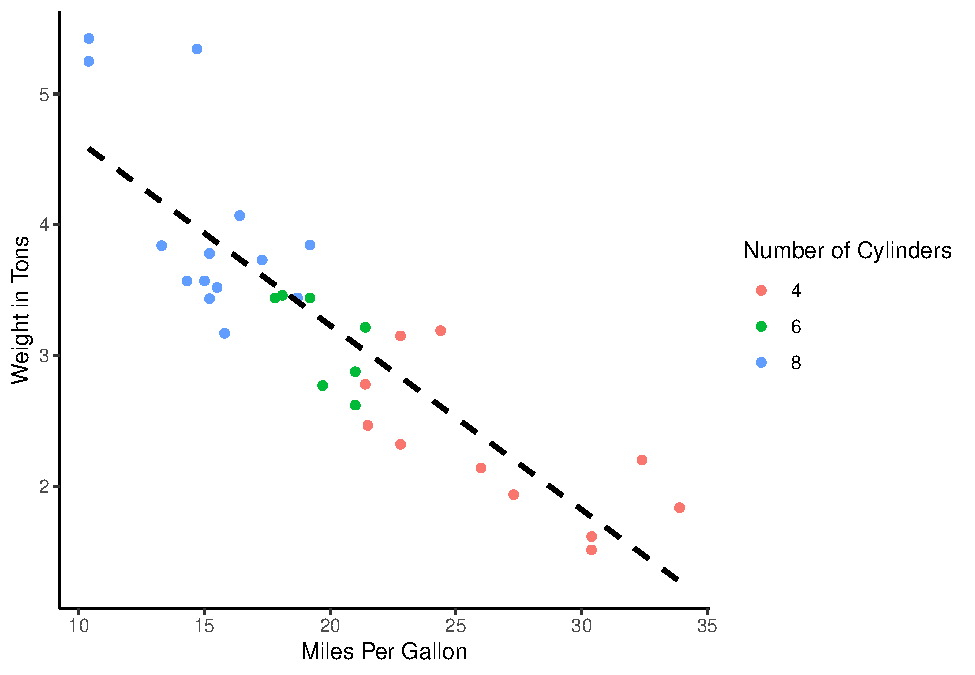
\includegraphics{C:/Users/Sven/Documents/Psychologie/master/markdown/output/apa7_document_files/figure-latex/method-example-fig-1.pdf}
\caption{\label{fig:method-example-fig}Plot of mpg over wt}
\end{figure}

You can also refer in inline code to data objects. We used the dataset \texttt{mtcars} for our analysis. It consists of data of 32 cars. The syntax ``r command'' in backticks will evaluate the command using your R-engine.

\hypertarget{results}{%
\section{Results}\label{results}}

Write your results here. You can add chunks for additional analysis. But to ensure readability, I would recommend conducting all anaylsis inside the appropriately named children.

You can cite R-packages used by calling the object \texttt{r\_citiations}. If you want to only cite R itself within your text, but refer to all packages used in a footnote, call \texttt{r\_citations\$r} in text and \texttt{r\_citations\$pkgs} after the end of the sentence. This report was generated using R {[}Version 4.1.3; R Core Team (\protect\hyperlink{ref-R-base}{2022}){]}\footnote{We, furthermore, used the R-packages \emph{knitr} (Version 1.41; \protect\hyperlink{ref-R-knitr}{Xie, 2015}), \emph{papaja} (Version 0.1.1; \protect\hyperlink{ref-R-papaja}{Aust \& Barth, 2022}), and \emph{tidyverse} (Version 1.3.2; \protect\hyperlink{ref-R-tidyverse}{Wickham et al., 2019}).}.

You can print tables using the wonderful \texttt{apa\_table} command provided to you by \texttt{papaja} (see Table \ref{tab:results-example-table}). Here it is best to set the caption using the \texttt{caption} argument provided by \texttt{apa\_table()}.

\begin{table}[tbp]

\begin{center}
\begin{threeparttable}

\caption{\label{tab:results-example-table}The top five cars by Miles Per Gallon (MPG)}

\begin{tabular}{lll}
\toprule
car & \multicolumn{1}{c}{mpg} & \multicolumn{1}{c}{disp}\\
\midrule
Pontiac Firebird & 19.20 & 400.00\\
Hornet Sportabout & 18.70 & 360.00\\
Merc 450SL & 17.30 & 275.80\\
Merc 450SE & 16.40 & 275.80\\
Ford Pantera L & 15.80 & 351.00\\
\bottomrule
\addlinespace
\end{tabular}

\begin{tablenotes}[para]
\normalsize{\textit{Note.} This table was generated using papaja::apa\_table()}
\end{tablenotes}

\end{threeparttable}
\end{center}

\end{table}

As you can see, the best car is Pontiac Firebird.

\hypertarget{discussion}{%
\section{Discussion}\label{discussion}}

Here you can discuss your results.

\newpage

\hypertarget{references}{%
\section{References}\label{references}}

\hypertarget{refs}{}
\begin{CSLReferences}{1}{0}
\leavevmode\vadjust pre{\hypertarget{ref-R-papaja}{}}%
Aust, F., \& Barth, M. (2022). \emph{{papaja}: {Prepare} reproducible {APA} journal articles with {R Markdown}}. \url{https://github.com/crsh/papaja}

\leavevmode\vadjust pre{\hypertarget{ref-R-base}{}}%
R Core Team. (2022). \emph{R: A language and environment for statistical computing}. R Foundation for Statistical Computing. \url{https://www.R-project.org/}

\leavevmode\vadjust pre{\hypertarget{ref-R-tidyverse}{}}%
Wickham, H., Averick, M., Bryan, J., Chang, W., McGowan, L. D., François, R., Grolemund, G., Hayes, A., Henry, L., Hester, J., Kuhn, M., Pedersen, T. L., Miller, E., Bache, S. M., Müller, K., Ooms, J., Robinson, D., Seidel, D. P., Spinu, V., \ldots{} Yutani, H. (2019). Welcome to the {tidyverse}. \emph{Journal of Open Source Software}, \emph{4}(43), 1686. \url{https://doi.org/10.21105/joss.01686}

\leavevmode\vadjust pre{\hypertarget{ref-R-knitr}{}}%
Xie, Y. (2015). \emph{Dynamic documents with {R} and knitr} (2nd ed.). Chapman; Hall/CRC. \url{https://yihui.org/knitr/}

\end{CSLReferences}

\newpage

\hypertarget{appendix-appendix}{%
\appendix}


\hypertarget{talking-about-appendices}{%
\section{Talking about appendices}\label{talking-about-appendices}}

First-level headers create appendix-sections labelled A-Z. You can print tables here aswell and refer to them in your main part. They will receive a prefix to their Table/Figure Number based on the appendix section they are in (see Table \ref{tab:appendix-example}).

\begin{table}[tbp]

\begin{center}
\begin{threeparttable}

\caption{\label{tab:appendix-example}Best car only}

\begin{tabular}{lll}
\toprule
car & \multicolumn{1}{c}{mpg} & \multicolumn{1}{c}{disp}\\
\midrule
Pontiac Firebird & 19.20 & 400.00\\
\bottomrule
\end{tabular}

\end{threeparttable}
\end{center}

\end{table}

\hypertarget{another-section}{%
\section{Another section}\label{another-section}}

this creates another appendix section


\end{document}
